\section{Battery State of Charge}
Battery state of charge (SOC) also plays a large role in the bus charge problem. As a bus traverses a route, energy is discharged from the battery. If the battery state of charge drops to zero, the bus will power down and become unresponsive. It is therefore important to track battery charge levels when scheduling charge times.
\par Furthermore, as no charge actions are available while on route, SOC values are only tracked when in the charge station. Because these in-station time periods are also represented by the charge nodes from figure \ref{fig:busAvailEncode}, the two are in one-one correspondence. Consequently, every charge node$_{i,k}$ can be associated with an SOC value, denoted $d_{i,k}$ as shown in figure \ref{fig:socDiagram}.  
\begin{figure}
	\centering
	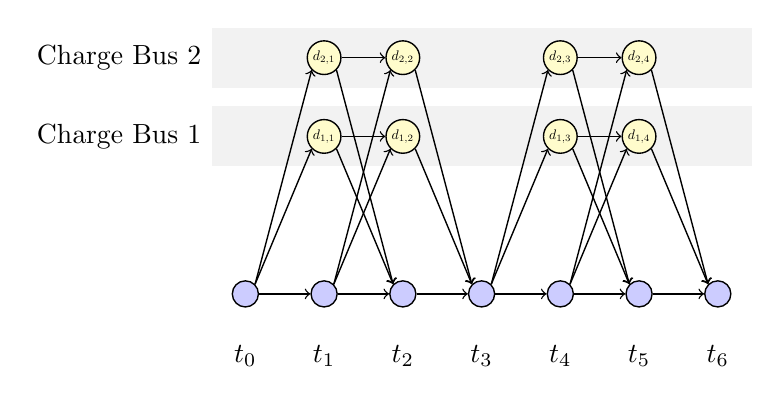
\begin{tikzpicture} 

		\node[rectangle, fill=gray!10, minimum width=2.7in, minimum height=.3in,label=left:Charge Bus 2](bus2Box) at (3,3){};
		\node[rectangle, fill=gray!10, minimum width=2.7in, minimum height=.3in,label=left:Charge Bus 1](bus1Box) at (3,2){};

		\node[circle, fill=blue!20, line width=0.5pt, draw=black, minimum size=0.1in](one) at (0,0){};
		\node[circle, fill=blue!20, line width=0.5pt, draw=black, minimum size=0.1in](two) at (1,0){}; 
		\node[circle, fill=blue!20, line width=0.5pt, draw=black, minimum size=0.1in](three) at (2,0){};
		\node[circle, fill=blue!20, line width=0.5pt, draw=black, minimum size=0.1in](four) at (3,0){};
		\node[circle, fill=blue!20, line width=0.5pt, draw=black, minimum size=0.1in](five) at (4,0){};
		\node[circle, fill=blue!20, line width=0.5pt, draw=black, minimum size=0.1in](six) at (5,0){};
		\node[circle, fill=blue!20, line width=0.5pt, draw=black, minimum size=0.1in](seven) at (6,0){};
		
		\node[circle, fill=yellow!20, line width=0.5pt, draw=black, minimum size=0.1in, inner sep=1pt](eight) at (1,2){\scalebox{0.5}{$d_{1,1}$}};
		\node[circle, fill=yellow!20, line width=0.5pt, draw=black, minimum size=0.1in, inner sep=1pt](nine) at (2,2){\scalebox{0.5}{$d_{1,2}$}};
		\node[circle, fill=yellow!20, line width=0.5pt, draw=black, minimum size=0.1in, inner sep=1pt](ten) at (4,2){\scalebox{0.5}{$d_{1,3}$}}; 
		\node[circle, fill=yellow!20, line width=0.5pt, draw=black, minimum size=0.1in, inner sep=1pt](eleven) at (5,2){\scalebox{0.5}{$d_{1,4}$}}; 

		\node[circle, fill=yellow!20, line width=0.5pt, draw=black, minimum size=0.1in, inner sep=1pt](twelve) at (1,3){\scalebox{0.5}{$d_{2,1}$}};
		\node[circle, fill=yellow!20, line width=0.5pt, draw=black, minimum size=0.1in, inner sep=1pt](thirteen) at (2,3){\scalebox{0.5}{$d_{2,2}$}};
		\node[circle, fill=yellow!20, line width=0.5pt, draw=black, minimum size=0.1in, inner sep=1pt](fourteen) at (4,3){\scalebox{0.5}{$d_{2,3}$}}; 
		\node[circle, fill=yellow!20, line width=0.5pt, draw=black, minimum size=0.1in, inner sep=1pt](fifteen) at (5,3){\scalebox{0.5}{$d_{2,4}$}}; 

		\draw [->, line width=0.5pt] (one.east) -- (two.west);
		\draw [->, line width=0.5pt] (two.east) -- (three.west);
		\draw [->, line width=0.5pt] (three.east) -- (four.west);
		\draw [->, line width=0.5pt] (four.east) -- (five.west);
		\draw [->, line width=0.5pt] (five.east) -- (six.west);
		\draw [->, line width=0.5pt] (six.east) -- (seven.west);

		\draw [->, line width=0.5pt] (one.north east) -- (eight.south west);
		\draw [->, line width=0.5pt] (two.north east) -- (nine.south west);
		\draw [->, line width=0.5pt] (four.north east) -- (ten.south west);
		\draw [->, line width=0.5pt] (five.north east) -- (eleven.south west);
		\draw [->, line width=0.5pt] (eight.south east) -- (three.north west);
		\draw [->, line width=0.5pt] (nine.south east) -- (four.north west);
		\draw [->, line width=0.5pt] (ten.south east) -- (six.north west);
		\draw [->, line width=0.5pt] (eleven.south east) -- (seven.north west);
		\draw [->, line width=0.5pt] (eight.east) -- (nine.west);
		\draw [->, line width=0.5pt] (ten.east) -- (eleven.west); 

		\draw [->, line width=0.5pt] (one.north east) -- (twelve.south west);
		\draw [->, line width=0.5pt] (two.north east) -- (thirteen.south west);
		\draw [->, line width=0.5pt] (four.north east) -- (fourteen.south west);
		\draw [->, line width=0.5pt] (five.north east) -- (fifteen.south west);
		\draw [->, line width=0.5pt] (twelve.south east) -- (three.north west);
		\draw [->, line width=0.5pt] (thirteen.south east) -- (four.north west);
		\draw [->, line width=0.5pt] (fourteen.south east) -- (six.north west);
		\draw [->, line width=0.5pt] (fifteen.south east) -- (seven.north west);
		\draw [->, line width=0.5pt] (twelve.east) -- (thirteen.west);
		\draw [->, line width=0.5pt] (fourteen.east) -- (fifteen.west); 

		\node[rectangle, minimum width=0.3in, minimum height=1.2in,label=below:$t_0$](time0Box) at (0,1){};
		\node[rectangle, minimum width=0.3in, minimum height=1.2in,label=below:$t_1$](time1Box) at (1,1){};
		\node[rectangle, minimum width=0.3in, minimum height=1.2in,label=below:$t_2$](time2Box) at (2,1){};
		\node[rectangle, minimum width=0.3in, minimum height=1.2in,label=below:$t_3$](time3Box) at (3,1){};
		\node[rectangle, minimum width=0.3in, minimum height=1.2in,label=below:$t_4$](time4Box) at (4,1){};
		\node[rectangle, minimum width=0.3in, minimum height=1.2in,label=below:$t_5$](time5Box) at (5,1){};
		\node[rectangle, minimum width=0.3in, minimum height=1.2in,label=below:$t_6$](time6Box) at (6,1){}; 
	\end{tikzpicture}
	\caption{SOC indicators}
	\label{fig:socDiagram}
\end{figure}


\par Charge level progression between $d_{i,k}$ and $d_{i,k+1}$ is influenced by two factors: discharging on route, and charging. The route discharge, denoted $\delta$, represents the energy drawn from the battery in kWh.  When a bus returns from a route, the change in SOC is computed as 
\begin{align}
	d_{i,k+1} = d_{i,k} - \delta_i
\end{align}
where $\delta_i$ is the discharge for Bus $i$'s route as seen in figure \ref{fig:graphDelta}.  
\begin{figure}
	\centering
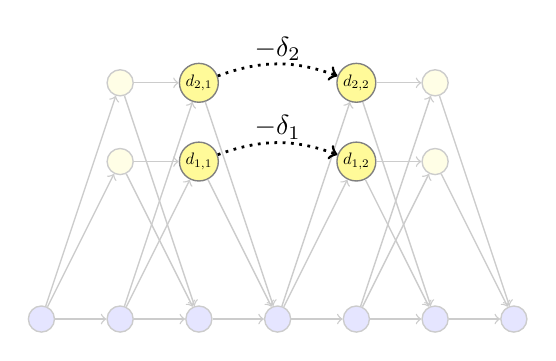
\begin{tikzpicture}
	\node[circle, fill=blue!10, line width=0.5pt, draw=black!20, minimum size=0.1in](one) at (0,0){};
	\node[circle, fill=blue!10, line width=0.5pt, draw=black!20, minimum size=0.1in](two) at (1,0){}; 
	\node[circle, fill=blue!10, line width=0.5pt, draw=black!20, minimum size=0.1in](three) at (2,0){};
	\node[circle, fill=blue!10, line width=0.5pt, draw=black!20, minimum size=0.1in](four) at (3,0){};
	\node[circle, fill=blue!10, line width=0.5pt, draw=black!20, minimum size=0.1in](five) at (4,0){};
	\node[circle, fill=blue!10, line width=0.5pt, draw=black!20, minimum size=0.1in](six) at (5,0){};
	\node[circle, fill=blue!10, line width=0.5pt, draw=black!20, minimum size=0.1in](seven) at (6,0){};
	
	\node[circle, fill=yellow!10, line width=0.5pt, draw=black!20, minimum size=0.1in](eight) at (1,2){};
	\node[circle, fill=yellow!40, line width=0.5pt, draw=black!50, minimum size=0.1in, inner sep=1pt](nine) at (2,2){\scalebox{0.6}{$d_{1,1}$}};
	\node[circle, fill=yellow!40, line width=0.5pt, draw=black!50, minimum size=0.1in, inner sep=1pt](ten) at (4,2){\scalebox{0.6}{$d_{1,2}$}};
	\node[circle, fill=yellow!10, line width=0.5pt, draw=black!20, minimum size=0.1in](eleven) at (5,2){};

	\node[circle, fill=yellow!10, line width=0.5pt, draw=black!20, minimum size=0.1in](twelve) at (1,3){};
	\node[circle, fill=yellow!40, line width=0.5pt, draw=black!50, minimum size=0.1in, inner sep=1pt](thirteen) at (2,3){\scalebox{0.6}{$d_{2,1}$}};
	\node[circle, fill=yellow!40, line width=0.5pt, draw=black!50, minimum size=0.1in, inner sep=1pt](fourteen) at (4,3){\scalebox{0.6}{$d_{2,2}$}};
	\node[circle, fill=yellow!10, line width=0.5pt, draw=black!20, minimum size=0.1in](fifteen) at (5,3){};

	\draw [->, line width=0.5pt, color=black!20] (one) -- (two);
	\draw [->, line width=0.5pt, color=black!20] (two) -- (three);
	\draw [->, line width=0.5pt, color=black!20] (three) -- (four);
	\draw [->, line width=0.5pt, color=black!20] (four) -- (five);
	\draw [->, line width=0.5pt, color=black!20] (five) -- (six);
	\draw [->, line width=0.5pt, color=black!20] (six) -- (seven);

	\draw [->, line width=0.5pt, color=black!20] (one) -- (eight);
	\draw [->, line width=0.5pt, color=black!20] (two) -- (nine);
	\draw [->, line width=0.5pt, color=black!20] (four) -- (ten);
	\draw [->, line width=0.5pt, color=black!20] (five) -- (eleven);
	\draw [->, line width=0.5pt, color=black!20] (eight) -- (three);
	\draw [->, line width=0.5pt, color=black!20] (nine) -- (four);
	\draw [->, line width=0.5pt, color=black!20] (ten) -- (six);
	\draw [->, line width=0.5pt, color=black!20] (eleven) -- (seven);
	\draw [->, line width=0.5pt, color=black!20] (eight)-- (nine);
	\draw [->, line width=0.5pt, color=black!20] (ten)-- (eleven); 

	\draw [->, line width=0.5pt, color=black!20] (one) -- (twelve);
	\draw [->, line width=0.5pt, color=black!20] (two) -- (thirteen);
	\draw [->, line width=0.5pt, color=black!20] (four) -- (fourteen);
	\draw [->, line width=0.5pt, color=black!20] (five) -- (fifteen);
	\draw [->, line width=0.5pt, color=black!20] (twelve) -- (three);
	\draw [->, line width=0.5pt, color=black!20] (thirteen) -- (four);
	\draw [->, line width=0.5pt, color=black!20] (fourteen) -- (six);
	\draw [->, line width=0.5pt, color=black!20] (fifteen) -- (seven);
	\draw [->, line width=0.5pt, color=black!20] (twelve)-- (thirteen);
	\draw [->, line width=0.5pt, color=black!20] (fourteen) -- (fifteen);
	\draw [dotted, color=black,-,line width=1pt] (nine) edge[->,bend left=20pt]node[above=-2.5pt]{\scalebox{1}{$-\delta_1$}}(ten); 
	\draw [dotted, color=black,-,line width=1pt] (thirteen) edge[->,bend left=20pt]node[above=-2.5pt]{\scalebox{1}{$-\delta_2$}}(fourteen); 

\end{tikzpicture}
	\caption{Relationship between exit nodes (left) and entrance nodes (right) as $\delta$}
	\label{fig:graphDelta}
\end{figure} 

\par When a charger connects to a bus, the increase or \textit{gain} in $d_{i,k}$ is denoted $g_{i,k}$, where $i$ and $k$ represent the respective bus and outgoing node indices. Figure \ref{fig:dSocDiagram} gives an example where $g_{1,1}$ and $g_{1,3}$ correspond to Bus 1's gain from $t_0$ to $t_1$ and $t_4$ to $t_5$.  
\begin{figure}
	\centering
	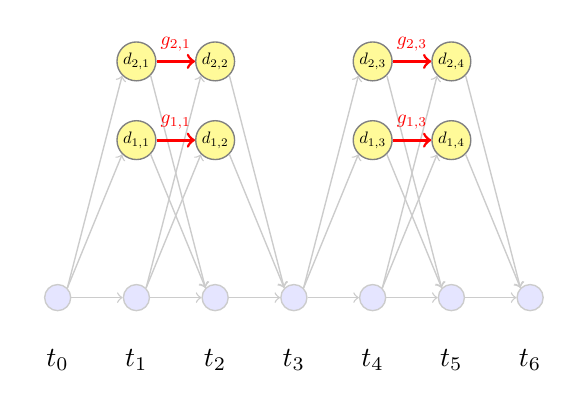
\begin{tikzpicture} 
		\node[circle, fill=blue!10, line width=0.5pt, draw=black!20, minimum size=0.1in](one) at (0,0){};
		\node[circle, fill=blue!10, line width=0.5pt, draw=black!20, minimum size=0.1in](two) at (1,0){}; 
		\node[circle, fill=blue!10, line width=0.5pt, draw=black!20, minimum size=0.1in](three) at (2,0){};
		\node[circle, fill=blue!10, line width=0.5pt, draw=black!20, minimum size=0.1in](four) at (3,0){};
		\node[circle, fill=blue!10, line width=0.5pt, draw=black!20, minimum size=0.1in](five) at (4,0){};
		\node[circle, fill=blue!10, line width=0.5pt, draw=black!20, minimum size=0.1in](six) at (5,0){};
		\node[circle, fill=blue!10, line width=0.5pt, draw=black!20, minimum size=0.1in](seven) at (6,0){};
		
		\node[circle, fill=yellow!40, line width=0.5pt, draw=black!50, minimum size=0.1in, inner sep=1pt](eight) at (1,2){\scalebox{0.6}{$d_{1,1}$}};
		\node[circle, fill=yellow!40, line width=0.5pt, draw=black!50, minimum size=0.1in, inner sep=1pt](nine) at (2,2){\scalebox{0.6}{$d_{1,2}$}};
		\node[circle, fill=yellow!40, line width=0.5pt, draw=black!50, minimum size=0.1in, inner sep=1pt](ten) at (4,2){\scalebox{0.6}{$d_{1,3}$}};
		\node[circle, fill=yellow!40, line width=0.5pt, draw=black!50, minimum size=0.1in, inner sep=1pt](eleven) at (5,2){\scalebox{0.6}{$d_{1,4}$}};

		\node[circle, fill=yellow!40, line width=0.5pt, draw=black!50, minimum size=0.1in, inner sep=1pt](twelve) at (1,3){\scalebox{0.6}{$d_{2,1}$}};
		\node[circle, fill=yellow!40, line width=0.5pt, draw=black!50, minimum size=0.1in, inner sep=1pt](thirteen) at (2,3){\scalebox{0.6}{$d_{2,2}$}};
		\node[circle, fill=yellow!40, line width=0.5pt, draw=black!50, minimum size=0.1in, inner sep=1pt](fourteen) at (4,3){\scalebox{0.6}{$d_{2,3}$}};
		\node[circle, fill=yellow!40, line width=0.5pt, draw=black!50, minimum size=0.1in, inner sep=1pt](fifteen) at (5,3){\scalebox{0.6}{$d_{2,4}$}};

		\draw [->, line width=0.5pt, color=black!20] (one.east) -- (two.west);
		\draw [->, line width=0.5pt, color=black!20] (two.east) -- (three.west);
		\draw [->, line width=0.5pt, color=black!20] (three.east) -- (four.west);
		\draw [->, line width=0.5pt, color=black!20] (four.east) -- (five.west);
		\draw [->, line width=0.5pt, color=black!20] (five.east) -- (six.west);
		\draw [->, line width=0.5pt, color=black!20] (six.east) -- (seven.west);

		\draw [->, line width=0.5pt, color=black!20] (one.north east) -- (eight.south west);
		\draw [->, line width=0.5pt, color=black!20] (two.north east) -- (nine.south west);
		\draw [->, line width=0.5pt, color=black!20] (four.north east) -- (ten.south west);
		\draw [->, line width=0.5pt, color=black!20] (five.north east) -- (eleven.south west);
		\draw [->, line width=0.5pt, color=black!20] (eight.south east) -- (three.north west);
		\draw [->, line width=0.5pt, color=black!20] (nine.south east) -- (four.north west);
		\draw [->, line width=0.5pt, color=black!20] (ten.south east) -- (six.north west);
		\draw [->, line width=0.5pt, color=black!20] (eleven.south east) -- (seven.north west);

		\draw [->, line width=0.5pt, color=black!20] (one.north east) -- (twelve.south west);
		\draw [->, line width=0.5pt, color=black!20] (two.north east) -- (thirteen.south west);
		\draw [->, line width=0.5pt, color=black!20] (four.north east) -- (fourteen.south west);
		\draw [->, line width=0.5pt, color=black!20] (five.north east) -- (fifteen.south west);
		\draw [->, line width=0.5pt, color=black!20] (twelve.south east) -- (three.north west);
		\draw [->, line width=0.5pt, color=black!20] (thirteen.south east) -- (four.north west);
		\draw [->, line width=0.5pt, color=black!20] (fourteen.south east) -- (six.north west);
		\draw [->, line width=0.5pt, color=black!20] (fifteen.south east) -- (seven.north west);
		\draw [->, line width=1pt, color=red] (twelve.east) -- node[above]{\scalebox{0.7}{$g_{2,1}$}}(thirteen.west);
		\draw [->, line width=1pt, color=red] (fourteen.east) -- node[above]{\scalebox{0.7}{$g_{2,3}$}}(fifteen.west); 
		\draw [->, line width=1pt, color=red] (eight.east) -- node[above]{\scalebox{0.7}{$g_{1,1}$}}(nine.west);
		\draw [->, line width=1pt, color=red] (ten.east) -- node[above]{\scalebox{0.7}{$g_{1,3}$}}(eleven.west); 

		\node[rectangle, minimum width=0.3in, minimum height=1.2in,label=below:$t_0$](time0Box) at (0,1){};
		\node[rectangle, minimum width=0.3in, minimum height=1.2in,label=below:$t_1$](time1Box) at (1,1){};
		\node[rectangle, minimum width=0.3in, minimum height=1.2in,label=below:$t_2$](time2Box) at (2,1){};
		\node[rectangle, minimum width=0.3in, minimum height=1.2in,label=below:$t_3$](time3Box) at (3,1){};
		\node[rectangle, minimum width=0.3in, minimum height=1.2in,label=below:$t_4$](time4Box) at (4,1){};
		\node[rectangle, minimum width=0.3in, minimum height=1.2in,label=below:$t_5$](time5Box) at (5,1){};
		\node[rectangle, minimum width=0.3in, minimum height=1.2in,label=below:$t_6$](time6Box) at (6,1){}; 

	\end{tikzpicture}
	\caption{Depiction of which edges increase SOC for the single rate case}
	\label{fig:dSocDiagram}
\end{figure}



Using a single charge rate however has drawbacks. If the rate is high, buses will charge quickly but the load on the grid will increase.  Decreased charge rates will stress the grid less but increase charge time. To address both situations, a method with additional flexibility must be used where both high and low charge rates are available. 
\par Let $g_{i,k,l}$ be the gain, where $i$ and $k$ represent the bus and outgoing node indicies as before and $l$ represents the charge rate index. Each charge rate index corresponds to an edge in the graph. Figure \ref{fig:multirateChargeEdges} gives an example where there are three rate options. Each rate corresponds to an edge between two charge nodes and together, all three edges provide multiple options for charging.
\begin{figure}
	\centering
	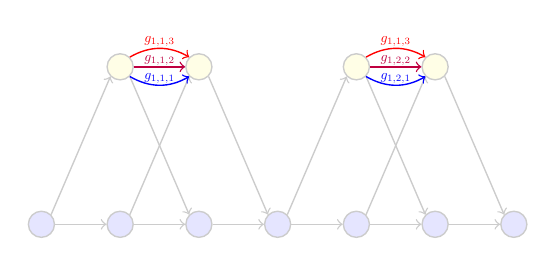
\begin{tikzpicture}[->, line width=0.5pt]
		\node[circle, fill=blue!10, draw=black!20,line width=0.5pt, minimum size=0.1in](one) at (0,0){};
		\node[circle, fill=blue!10, draw=black!20,line width=0.5pt, minimum size=0.1in](two) at (1,0){}; 
		\node[circle, fill=blue!10, draw=black!20,line width=0.5pt, minimum size=0.1in](three) at (2,0){};
		\node[circle, fill=blue!10, draw=black!20,line width=0.5pt, minimum size=0.1in](four) at (3,0){};
		\node[circle, fill=blue!10, draw=black!20,line width=0.5pt, minimum size=0.1in](five) at (4,0){};
		\node[circle, fill=blue!10, draw=black!20,line width=0.5pt, minimum size=0.1in](six) at (5,0){};
		\node[circle, fill=blue!10, draw=black!20,line width=0.5pt, minimum size=0.1in](seven) at (6,0){};
		\node[circle, fill=yellow!10, draw=black!20,line width=0.5pt, minimum size=0.1in](eight) at (1,2){};
		\node[circle, fill=yellow!10, draw=black!20,line width=0.5pt, minimum size=0.1in](nine) at (2,2){};
		\node[circle, fill=yellow!10, draw=black!20,line width=0.5pt, minimum size=0.1in](ten) at (4,2){}; 
		\node[circle, fill=yellow!10, draw=black!20,line width=0.5pt, minimum size=0.1in](eleven) at (5,2){}; 
		\draw [line width=0.5pt,color=black!20] (one.east) -- (two.west);
		\draw [line width=0.5pt,color=black!20] (two.east) -- (three.west);
		\draw [line width=0.5pt,color=black!20] (three.east) -- (four.west);
		\draw [line width=0.5pt,color=black!20] (four.east) -- (five.west);
		\draw [line width=0.5pt,color=black!20] (five.east) -- (six.west);
		\draw [line width=0.5pt,color=black!20] (six.east) -- (seven.west);
		\draw [line width=0.5pt,color=black!20] (one.north east) -- (eight.south west);
		\draw [line width=0.5pt,color=black!20] (two.north east) -- (nine.south west);
		\draw [line width=0.5pt,color=black!20] (four.north east) -- (ten.south west);
		\draw [line width=0.5pt,color=black!20] (five.north east) -- (eleven.south west);
		\draw [line width=0.5pt,color=black!20] (eight.south east) -- (three.north west);
		\draw [line width=0.5pt,color=black!20] (nine.south east) -- (four.north west);
		\draw [line width=0.5pt,color=black!20] (ten.south east) -- (six.north west);
		\draw [line width=0.5pt,color=black!20] (eleven.south east) -- (seven.north west);

		\draw [color=red,-,line width=0.5pt] (eight.north east) edge[->,bend left]node[above=-3pt]{\scalebox{0.5}{$g_{1,1,3}$}}(nine.north west);
		\draw [color=purple,line width=0.5pt] (eight.east) -- node[above=-3pt]{\scalebox{0.5}{$g_{1,1,2}$}}(nine.west);
		\draw [color=blue,-,line width=0.5pt] (eight.south east) edge[->, bend right]node[above=-3pt]{\scalebox{0.5}{$g_{1,1,1}$}}(nine.south west);

		\draw [color=red,-, line width=0.5pt] (ten.north east) edge[->, bend left]node[above=-3pt]{\scalebox{0.5}{$g_{1,1,3}$}}(eleven.north west);
		\draw [color=purple,line width=0.5pt] (ten.east) -- node[above=-3pt]{\scalebox{0.5}{$g_{1,2,2}$}}(eleven.west); 
		\draw [color=blue,-, line width=0.5pt] (ten.south east) edge[->, bend right]node[above=-3pt]{\scalebox{0.5}{$g_{1,2,1}$}}(eleven.south west);
	\end{tikzpicture}
	\caption{Multi-Rate Charging}
	\label{fig:multirateChargeEdges}
\end{figure} 

These gains are used to compute succeeding charge levels as 
\begin{align}\label{eqn:gainTotal}
	d_{i,k+1} = d_{i,k} +\sum_{l} g_{i,k,l},
\end{align} 
but because of group and flow constraints, only one charge rate can be active at a time. Therefore, $d_{i,k}$ can be expressed as 
\begin{align}\label{eqn:gainInitial}
	d_{i,k+1} = d_{i,k} + g_{i,k,l},
\end{align}
where the $l^{\text{th}}$ charge edge is active. 
\par $g_{i,k,l}$ is computed using the Constant Current Constant Voltage (CCCV) model as derived in \cite{whitaker_network_2021} which gives:
\begin{align}\label{eqn:CCCV}
	d_{i,k+1} = \bar{a}_ld_{i,k} - \bar{b}_lM 
\end{align}
Where $\bar{a}_l$ $\sim(0,1]$, depends on the charge rate and is experimentally determined, $M$ is the battery charge capacity in kWh, and $\bar{b}_l = \bar{a}_l - 1$.
Equations \ref{eqn:gainInitial} and \ref{eqn:CCCV} are used to show that
\begin{equation}\label{eqn:g}
\begin{aligned}
	& d_{i,k+1} = \bar{a}_ld_{i,k} - \bar{b}_lM \\ 
	\Rightarrow & d_{i,k+1} - d_{i,k} = \bar{a}_ld_{i,k} - \bar{b}_lM - d_{i,k}\\
	\Rightarrow & g_{i,k,l}  = \bar{a}_ld_{i,k} - \bar{b}_lM - d_{i,k}\\
	\Rightarrow & g_{i,k,l}  = (\bar{a}_l - 1)d_{i,k} - \bar{b_l}M\\
\end{aligned}
\end{equation}

The results from equation \ref{eqn:g}, however, only hold when a charger is connected to a bus, which is represented by a weight of $1$ for the edge corresponding to $g_{i,k,l}$. When the weight equals $0$, $g_{i,k,l}$ must also equal zero. These two situations can be described using a switching constraint known as the \textit{big M} technique. This technique is used to describe $g_{i,k,l}$ with equation \ref{eqn:g} when the transition weight is $1$ and $g_{i,k,l} = 0$ when $0$.
\begin{equation}\label{eqn:bigMIneq}
\begin{aligned}
	& \begin{dcases} 
		\begin{array}{l}
		g_{i,k,l} = d_{i,k}(\bar{a}_l - 1) - \bar{b}_lM
		\end{array} & x_{i,k,l} = 1\\
		\begin{array}{l}
		g_{i,k,l} = 0
		\end{array} & x_{i,k,l} = 0\\
	\end{dcases} \\ 
	\Rightarrow & 
	\begin{dcases} 
		\begin{array}{l}
		g_{i,k,l} \le d_{i,k}(\bar{a}_l - 1) - \bar{b}_lM\\
		g_{i,k,l} \ge d_{i,k}(\bar{a}_l - 1) - \bar{b}_lM\\
		\end{array}
		& x_{i,k,l} = 1 \\
		\begin{array}{l}
		g_{i,k,l} \le 0 \\
		g_{i,k,l} \ge 0 \\
		\end{array} & x_{i,k,l} = 0\\
    	\end{dcases} 
\end{aligned}
\end{equation}
where $x_{i,k,l}$ is the edge weight corresponding to $g_{i,k,l}$.  The piecewise function in equation \ref{eqn:bigMIneq} can be rewritten as 
\begin{equation}\label{eqn:bigM2}
 \begin{aligned} 
	 &\begin{dcases} 
		\begin{array}{l}
		g_{i,k,l} \le d_{i,k}(\bar{a}_l - 1) - \bar{b}_lM\\
		g_{i,k,l} \ge d_{i,k}(\bar{a}_l - 1) - \bar{b}_lM\\
		\end{array}
		& x_{i,k,l} = 1 \\
		\begin{array}{l}
		g_{i,k,l} \le 0 \\
		g_{i,k,l} \ge 0 \\
		\end{array} & x_{i,k,l} = 0\\ 
	\end{dcases} \\
	\Rightarrow & 
	 \begin{array}{l}
		 g_{i,k,l} \le d_{i,k}(\bar{a}_l - 1) - \bar{b}M - M(1 - x_{i,k,l})\\
		 g_{i,k,l} \ge d_{i,k}(\bar{a}_l - 1) - \bar{b}M\\
		 g_{i,k,l} \le 0 + Mx_{i,k,l} \\
		 g_{i,k,l} \ge 0 \\
	 \end{array}
\end{aligned}
\end{equation}
The results of equation \ref{eqn:bigM2} obtain a switching effect.  When $x_{i,k,l} = 1$, equation \ref{eqn:bigM2} becomes 
\begin{equation}
	\begin{aligned}
		\color{blue}{g_{i,k,l}}  &\color{blue}{\le d_{i,k}(\bar{a}_l - 1) - \bar{b}_lM} \\
		\color{blue}{g_{i,k,l}}  &\color{blue}{\ge d_{i,k}(\bar{a}_l - 1) - \bar{b}_lM} \\
		\color{red}{g_{i,k,l}} & \color{red}{\le M} \\
		\color{red}{g_{i,k,l}} & \color{red}{\ge 0}.  
	\end{aligned}
\end{equation}
The \textcolor{blue}{active constraints} imply equality for $g_{i,k,l}$ = $(\bar{a}_l - 1)d_{i,k} - \bar{b_l}M$.  The \textcolor{red}{inactive constraints} imply that $g_{i,k,l}$ is greater then zero, and less then the battery capacity.  These constraints are also true, but have no effect on $g_{i,k,l}$. When $x_{i,k,l} = 0$, equation \ref{eqn:bigM2} becomes
\begin{equation}
	\begin{aligned}
		\color{red}{g_{i,k,l}}  &\color{red}{\le d_{i,k}(\bar{a}_l - 1) - \bar{b}_lM - M} \\
		\color{red}{g_{i,k,l}}  &\color{red}{\ge d_{i,k}(\bar{a}_l - 1) - \bar{b}_lM} \\
		\color{blue}{g_{i,k,l}} &\color{blue}{\le 0} \\
		\color{blue}{g_{i,k,l}} &\color{blue}{\ge 0}.  
	\end{aligned}
\end{equation}
Where the \textcolor{red}{inactive constraints} indicate that $g_{i,k,l}$ is less then some positive value, and greater than a negative value. These constarints have no effect as the \textcolor{blue}{active constraints} imply equality for $g_{i,k,l} = 0$.

\par Equation \ref{eqn:bigM2} can be expressed in linear form as 
\begin{equation}\label{eqn:chargeConstraints}
	\begin{aligned} 
		-g_{i,k,l} + d_{i,k}(\bar{a}_l - 1) + x_{i,k,l} &\le M(\bar{b_l} + 1) \\
		 g_{i,k,l} - d_{i,k}(\bar{a}_l - 1)  &\le  - \bar{b_l}M \\
		 g_{i,k,l} - Mx_{i,k} &\le 0 \\
		-g_{i,k,l} &\le 0.  
	\end{aligned}
\end{equation} 
